\documentclass{article}
\usepackage{blindtext}
\usepackage{graphicx}
\usepackage{color}

\usepackage{polski}
\usepackage[utf8]{inputenc}

\usepackage[paperheight=4400pt, left=1.25in, right=1.25in, top=0.5in, bottom=0.4in]{geometry}


\setcounter{totalnumber}{100}

\title{Optymalizacja kombinatoryczna - sprawozdanie}
\date{}
\author{Sebastian Nawrot 145177 Bioinformatyka\\sebastian.nawrot@student.put.poznan.pl}

\pagenumbering{gobble}

\renewcommand{\familydefault}{\sfdefault}

\begin{document}

\maketitle


\section{Problem}
Dany jest spójny graf $G=(V, E)$ z wagami $w_{i}$ przypisanymi do każdej
krawędzi $v_{i}\in V$. Należy znaleźć ścieżkę łączącą wszystkie wierzchołki
(każdy odwiedzony minimum raz) taką, aby zminimalizować jej koszt $S$. Koszt
ten wyliczany jest dynamicznie w trakcie konstrukcji w taki sposób, że:

\renewcommand{\labelenumi}{\alph{enumi}.}
\begin{enumerate}
  \item stanowi sumę wszystkich wag odwiedzonych do tej pory krawędzi, oraz
  \item co $x$ odwiedzonych łuków licząc od startu do aktualnej sumy $S$ dodawana jest
  suma ostatnich $x/2$ odwiedzonych wag pomnożona przez podwójny stopień
  wierzchołka, w którym znajduje się algorytm przeszukiwania po przejściu $x$ krawędzi.
\end{enumerate}

\noindent
Założenia dla instancji problemu: można przyjąć początkowo: $\left| V \right|$
minimum: 100, $deg(v) = \left[1, 6\right]$, $w_{i} = \left[1, 100\right]$, $x$ = minimum 5.



\section{Opis algorytmu}

\renewcommand{\labelenumi}{2.\arabic{enumi}}
\begin{enumerate}
\item \large Wyszukiwanie pierwszego rozwiązania:\\ \normalsize\\
  Algorytm zaczyna od wyboru wierzchołka z najniższym indeksem, jest on dodawany
  do wektora przechowującego rozwiązanie. Następnie w pętli, z obecnego
  rozwiązania wybieramy ostatnio dodany wierzchołek i sprawdzamy czy sąsiaduje
  on z jakimkolwiek wierzchołkiem, którego jeszcze nie ma w rozwiązaniu. 
  
  - Jeżeli tak, dodajemy nieodwiedzony wierzchołek do rozwiązania i powtarzamy
  ten krok. Jeżeli istnieje kilka takich wierzchołków wybieramy ten, do którego
  prowadzi krawędź z najniższą wagą.
  \\- Jeżeli nie, wybieramy z rozwiązania jeszcze wcześniejszy
  wierzchołek i powtarzamy krok. Cofając się po ścieżce, po natrafieniu na
  nieodwiedzonego wcześniej sąsiada, dodajemy go w obecnym miejscu rozwiązania.
  W tym wypadku dodajemy także wierzchołek który do niego prowadził.
  
  Algorytm kończy działanie gdy wszystkie wierzchołki grafu znajdują się w rozwiązaniu.

\item \large Wyszukiwanie sąsiedztwa:\\ \normalsize\\
  Wyszukiwanie sąsiedztwa dla obecnego rozwiązania odbywa się poprzez wybór 2
  krawędzi i próbę zamiany ich kolejnośći, odwracając jednocześnie ścieżkę pomiędzy nimi.
  
  Przykładowo dla rozwiązania:
  \\1 - 2 - \textcolor{blue}{3 - 4 - 5 - 6} - 7 - 8
  
  wybieramy krawędzie 3 i 6 i odwracamy fragment pomiędzy nimi, powstaje w ten sposób:
  \\1 - 2 - \textcolor{red}{6 - 5 - 4 - 3} - 7 - 8

  Jeżeli ścieżki nie da się utworzyć, tzn. dla powyższego przykładu nie ma krawędzi
  pomiędzy wierzchołkami 2 - 6 i 3 - 7, wyszukujemy połączenia pomiędzy nimi.
  Szukanie tej ścieżki jest ograniczone, dobudowane połączenie może zawierać
  maksymalnie 3 wierzchołki, używamy do tego algorytmu przeszukiwania w głąb.

  Ilość sąsiedztw do wyszukania kontrolowana jest przez parametr wejściowy
  algorytmu. Na wstępie zwracane są sąsiedztwa, które nie wymagają dobudowy
  dodatkowej ścieżki, ponieważ to właśnie one w większości wypadków prowadzą
  do najlepszych rozwiązań. Jest ich na tyle mało (np. dla grafu ze 100
  wierzchołkami i ilością krawędzi 6-30 jest ich około 200) że dopiero w drugiej
  kolejności uzupełniamy je rozwiązanami z dobudowanymi połączeniami.

  Aktualizacja listy tabu odbywa się poprzez dodanie skrajnych wierzchołków
  zamienionego fragmentu, dla powyższego przykładu będzie to 3 i 6.

  \vspace{5mm}
  Nie jestem pewien czy jest to dobry sposób wyszukiwania sąsiedztw, zamiana
  kolejności fragmentów w istniejącej ścieżce wydaje mi się jedynym dobrym pomysłem.
  Niestety liczba takich możliwych podstawień jest dosyć mała a na laboratoriach
  była mowa o ograniczaniu ich ilości do kilku tysięcy, stąd próba zwiększenia
  ich ilości poprzez tworzenie losowych połączeń.
  

\item \large Działanie algorytmu:\\ \normalsize\\
  Na wstępie wyszukujemy pierwsze rozwiązanie używając funkcji opisanej w
  podpunkcie 2.1, oznaczamy je jako obecne rozwiązanie. Następnie przechodzimy
  do wykonywania głównej pętli algorytmu, wykonujemy ją przez ilość czasu
  podaną w parametrze wejściowym, domyślnie jest jedna minuta.

  W pętli wyszukujemy sąsiedztwa dla obecnego rozwiązania, ich ilość także
  kontrolowana jest przez parametr wejściowy. Ze zbioru wygenerowanych sąsiedztw
  wybieramy te, które najbardziej polepsza obecne rozwiązanie czyli te, 
  dla którego wartość funkcji celu jest najmniejsza. Ustawiamy je jako nasze
  obecne rozwiązanie.
  
  Jeżeli żadne z sąsiedztw nie polepsza obecnej ścieżki przechodzimy w tryb
  pogarszania rozwiązania przez ilość następnych iteracji określoną w kolejnym
  parametrze wejściowym. Następnie z powrotem przełączamy w tryb normalny i
  zaczynamy szukać polepszeń.


\item \large Dodatkowe elementy:\\ \normalsize\\
  W każdej iteracji pętli, zaraz po wybraniu najlepszego kandydata na następne
  rozwiązanie próbujemy polepszyć ścieżkę manualnie. Robimy to poprzez usunięcie
  z rozwiązania wierzchołków, które znajdują się w ścieżce dwa razy. Ponieważ
  generowanie sąsiedztwa poprzez dobudowanie fragmentów zwiększa długość ścieżki
  potrzebujemy czegoś co będzie w stanie ją skrócić. Algorytm ten jest bardzo
  prymitywny i pozostawia sporo do życzenia.

  Działanie polega na wyszukaniu wszystkich powtarzających się wierzchołków.
  Następnie, dla każdego z nich sprawdzamy czy po jego wycięciu możliwe jest
  odtworzenie ścieżki w jego miejscu tzn. czy wierzchołki po lewej i prawej
  stronie mają wspólną krawedź. Jeżeli tak usuwamy go, powtarzamy te operację
  aż do momentu gdy każdy z nich będzie występował tylko raz, lub gdy pomiędzy
  żadymi z sąsiednich wierzchołków nie będzie krawędzi.

  Naturalnym wydało mi się dodanie sprawdzenia czy po takiej operacji, nowo
  powstałe rozwiązanie jest lepsze od poprzedniego. Testy wykazały jednak, że
  prowadzi to do gorszych końcowych rozwiązań i jakiekolwiek skrócenie ścieżki
  jest lepsze od polepszenia wyniku funkcji celu.

  \vspace{5mm}
  Kolejnym sposobem na ulepszenie algoyrtmu było wykorzystanie wszystkich
  sąsiedztw wegenerowanych w obecnej iteracji i stworzenie z nich jednego,
  jeszcze lepszego rozwiązania. Jeżeli zmiany w sąsiedztwach nie pokrywały się,
  tzn. można było jednocześnie wykonać obydwa przekształcenia, sprawdzaliśmy czy
  generuje to lepsze rozwiązanie. Niestety, mimo tego, że w pierwszych kilku
  iteracjach wyniki były znacząco lepsze, to końcowe wyniki były gorsze. Z tego
  powodu zrezygnowałem z tej funkcjonalności.
\end{enumerate}



\section{Testowanie metaheurestyki}
W algorytmie, poza oczywistymi parametrami grafu, możemy przetestować następujące parametry:
\begin{itemize}
  \item Ilość iteracji, na którą ruch jest blokowany (dodawany do listy tabu)
  \item Ilość iteracji algorytmu w fazie pogarszającej rozwiązania
  \item Ilość sąsiedztw do wyszukania
  \item Czas wykonywania algorytmu
\end{itemize}


Podczas tworzenia algorytmu domyślnymi parametrami dla powyższych właściwości było
11 iteracji blokady, 8 iteracji pogarszania, 300 sąsiedztw, i 60 sekund trwania. 
Dla przykładowego grafu 100 wierzchołków 6-30 krawędzi, końcowe rozwiązanie było
średnio o 70\% lepsze względem pierwszego. Jest to dobry punkt odniesienia i
względem tych wartości będą wykonywane testy.

%\newpage
Wykres przedstawia wykonanie algorytmu dla powyższych wartości, wykonanie
całości trwało minutę. Możemy zauważyć, że algorytm działa poprawnie, tzn.
polepsza wartość funkcji celu i nie zapętla się wokół jednego rozwiązania.
Widać także, że w miarę upływu czasu efektywność spada i coraz ciężej znaleźć
rozwiązanie polepszające.

%\centering

\begin{center}
  \makebox[\linewidth]{
    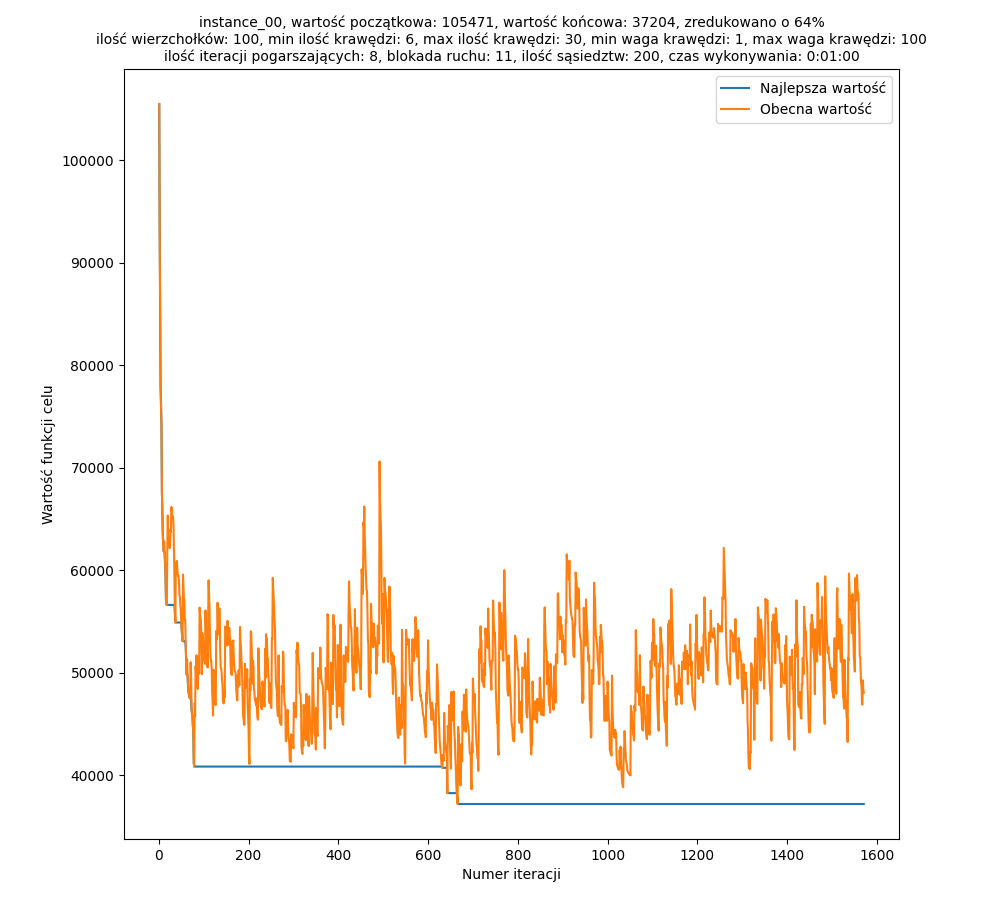
\includegraphics[scale=0.6]{wykres.png}
  }
\end{center}


%\newpage
\large\textf{Czas działania algorytmu:}\normalsize\\
Na poniższym wykresie przedstawiona jest uśredniona wartość funkcji celu
dla 100 instancji. Jak można zauważyć, po minucie poprawa jest znikoma.
Dla kolejnych testów jako czas wykonania przyjmiemy 60 sekund.


\begin{center}
  \makebox[\linewidth]{
    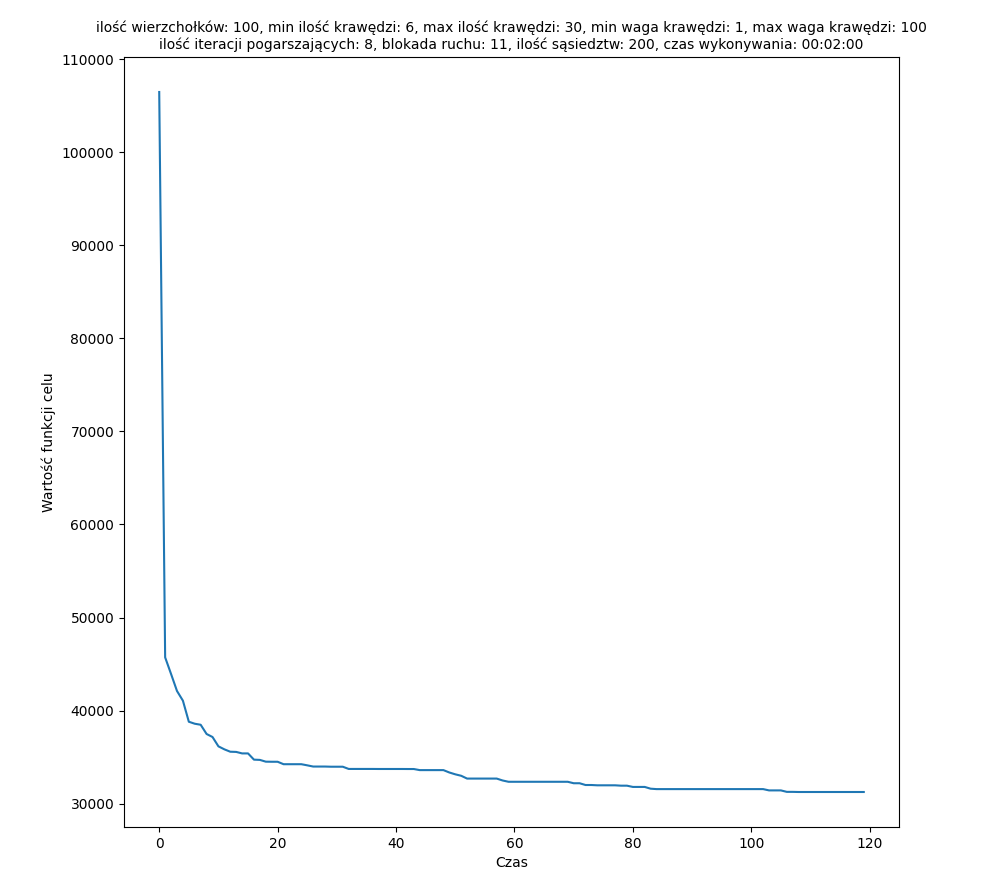
\includegraphics[scale=0.6]{czas_wykonania.png}
  }
\end{center}

\large\textbf{Wpływ ilości krawędzi na końcowe rozwiązanie:}\normalsize\\
Na poniższym wykresie przedstawiony jest uśredniony stopień polepszenia
wartości rozwiązania końcowego względem pierwszego wyrażony w procentach,
tzn. dla zakresu 38-44 początkowa wartość funkcji celu została zredukowana
o 93\%. Dla każdego zakresu krawędzi wygenerowano 100 instancji. Możemy
zauważyć, że istnieje zależność pomiędzy ilością krawędzi i stopniem poprawy
rozwiązania. Im więcej krawędzi, tym łatwiej znaleźć polepszające sąsiedztwo
co prowadzi do lepszych wyników końcowych.

\begin{center}
  \makebox[\linewidth]{
    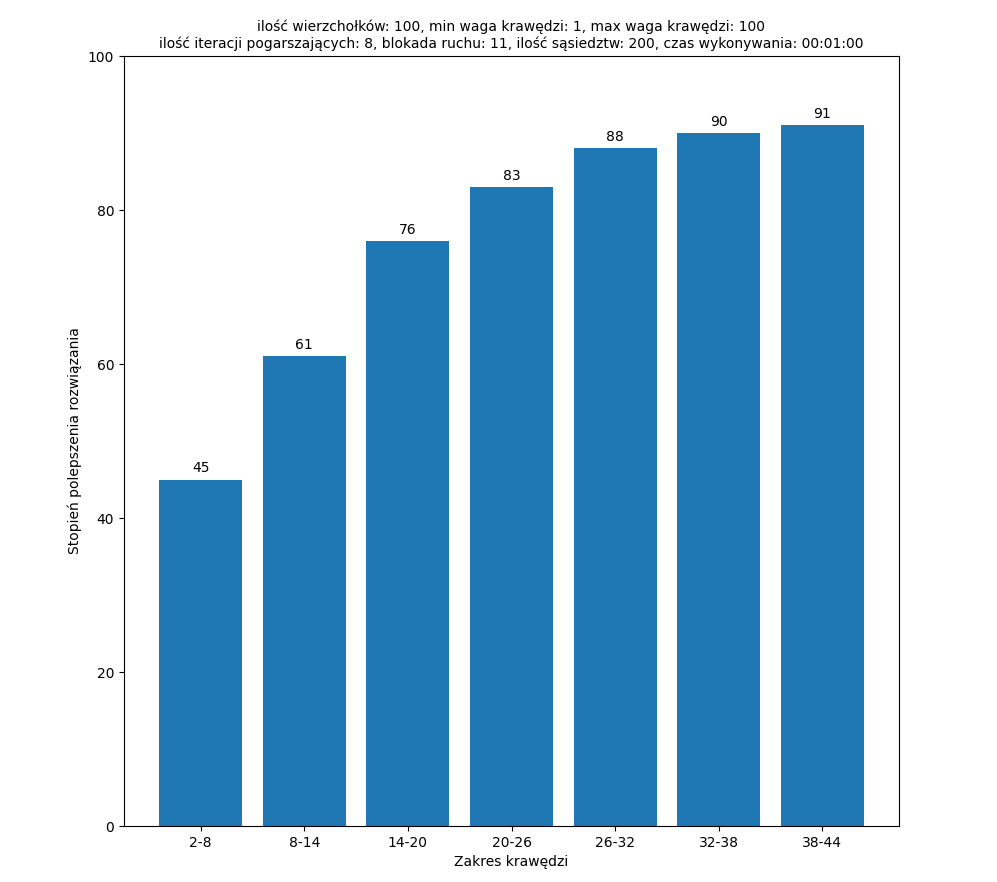
\includegraphics[scale=0.6]{krawedzie.png}
  }
\end{center}


\begin{center}
  \makebox[\linewidth]{
    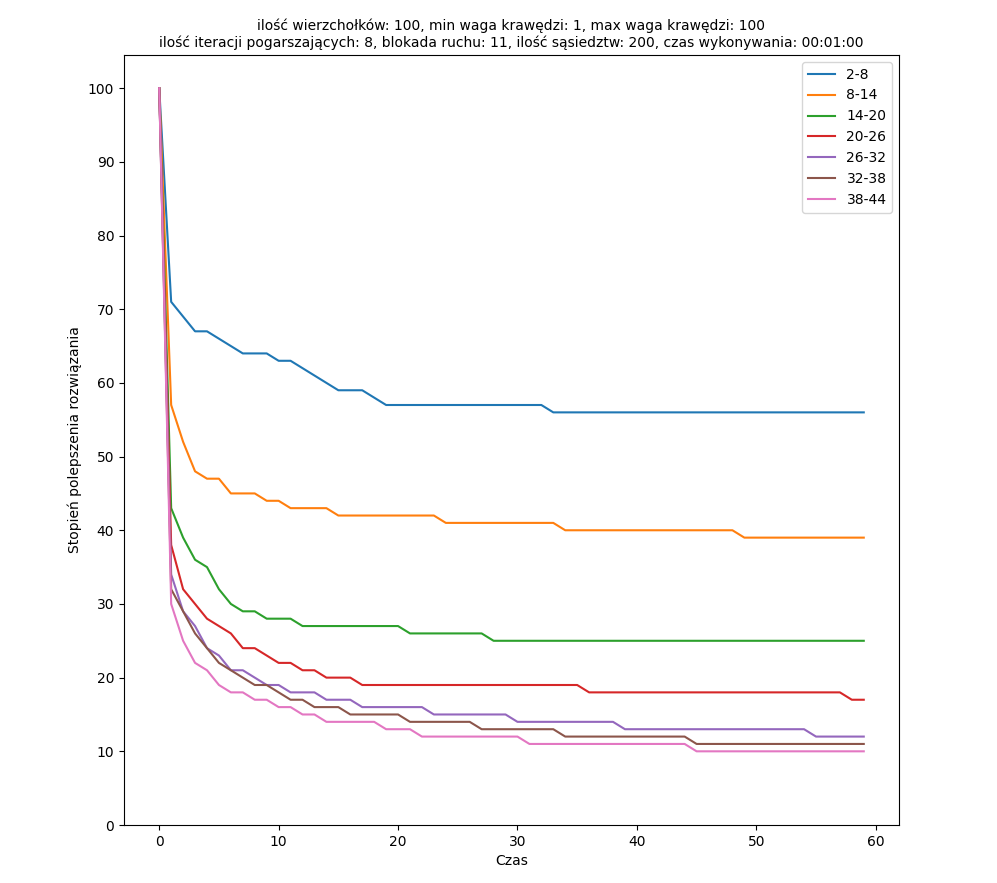
\includegraphics[scale=0.6]{krawedzie_wykres.png}
  }
\end{center}


\large\textbf{Wpływ ilości wyszukiwanych sąsiedztw na końcowe rozwiązanie:}\normalsize\\
Wykres przedstawia grupy instancji z różną ilością sąsiedztw generowanych
w jednej iteracji i ich wpływ na końcową wartość fukncji celu. Dla wartości
200 sąsiedztw uzyskujemy najlepsze rezultaty. Wynika to z że, dla parametrów
wygenerowanych grafów (100 wierzchołków, 6-30 krawędzi) ilość sąsiedztw
uzyskiwanych bez dobudowywania ścieżki do właśnie około 200. Wszystkie
sąsiedztwa powyżej tej wartości to ścieżki z losowo wybranymi wierzchołkami
i dobudowanymi połączeniami. Bardzo rzadko są w stanie coś polepszyć i z racji
60 sekund na wykonanie algorytmu ich generowanie jest marnowaniem czasu
na dodatkowe iteracje. Ze szczegółowych grafów poszczególnych instancji możemy
odczytać że przy 200 sąsiedztwach program wykonuje średnio około 600 iteracji
przez 60 sekund, dla 600 sąsiedztw jest to 150 iteracji, dla 1000 100, dla 1400 80
i dla 1800 około 70. Nie przekłada się to jednak całkowicie na wyniki na wykresie,
sąsiedztwa od 600 do 1800 znajdują się mnie więcej na tym samym poziomie. Nie
jestem w stanie określić dlaczego, aczkolwiek ukazuje to, że moduł dobierania
losowych ścieżek jest całkowicie bezużyteczny. Najlepszym sposobem na
ustawienie tego parametru jest jego całkowite usunięcie i wykorzystanie
wszystkich rozwiązań z pierwszej fazy szukania sąsiedztw.

\begin{center}
  \makebox[\linewidth]{
    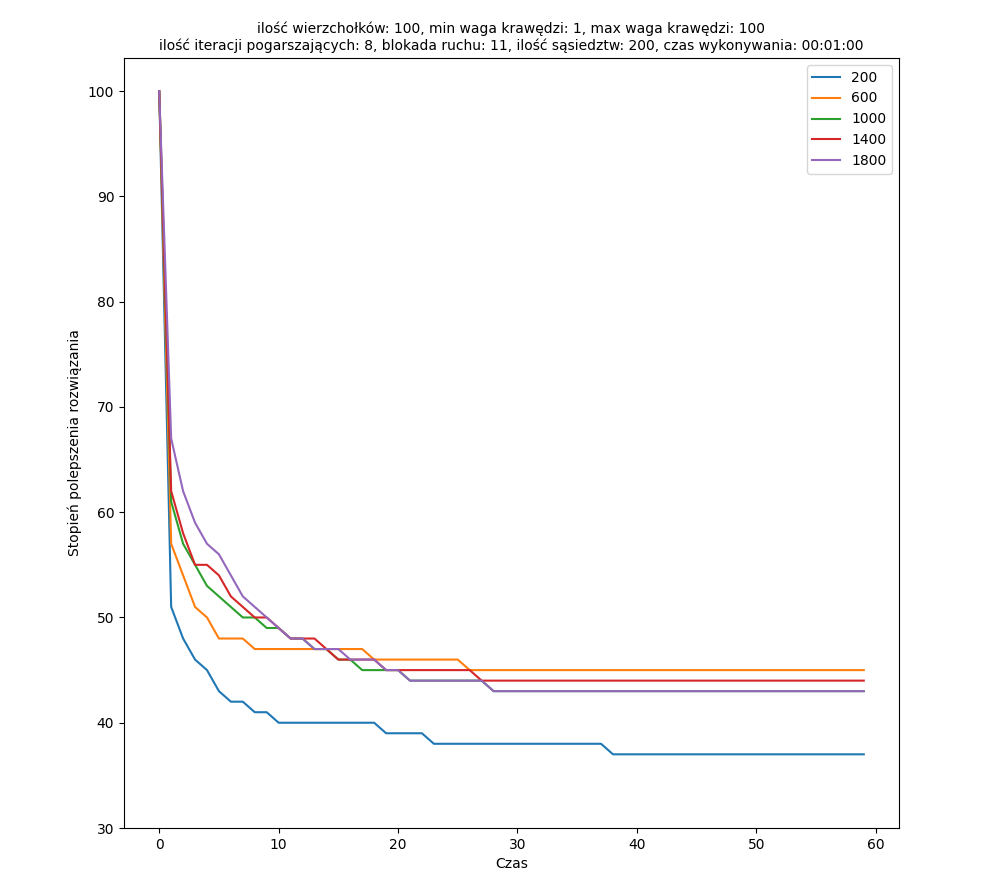
\includegraphics[scale=0.6]{sasiedztwa_wykres.png}
  }
\end{center}


\large\textbf{Wpływ ilości iteracji pogarszających rozwiązanie na końcowe rozwiązanie:}\normalsize\\
Wykres przedstawia zależność pomiędzy ilością iteracji pogarszających rozwiązanie
i stopniem polepszenia wartości funkcji celu. Wartość w okolicach 4 wydaje się
najlepszym wyborem dla tego parametru. Wartości dla testu mają zbyt duży rozkład,
warto byłoby przeprowadzić kolejny test z wartościam od 1 do 8 aby poznać
najlepszą wartość.


\begin{center}
  \makebox[\linewidth]{
    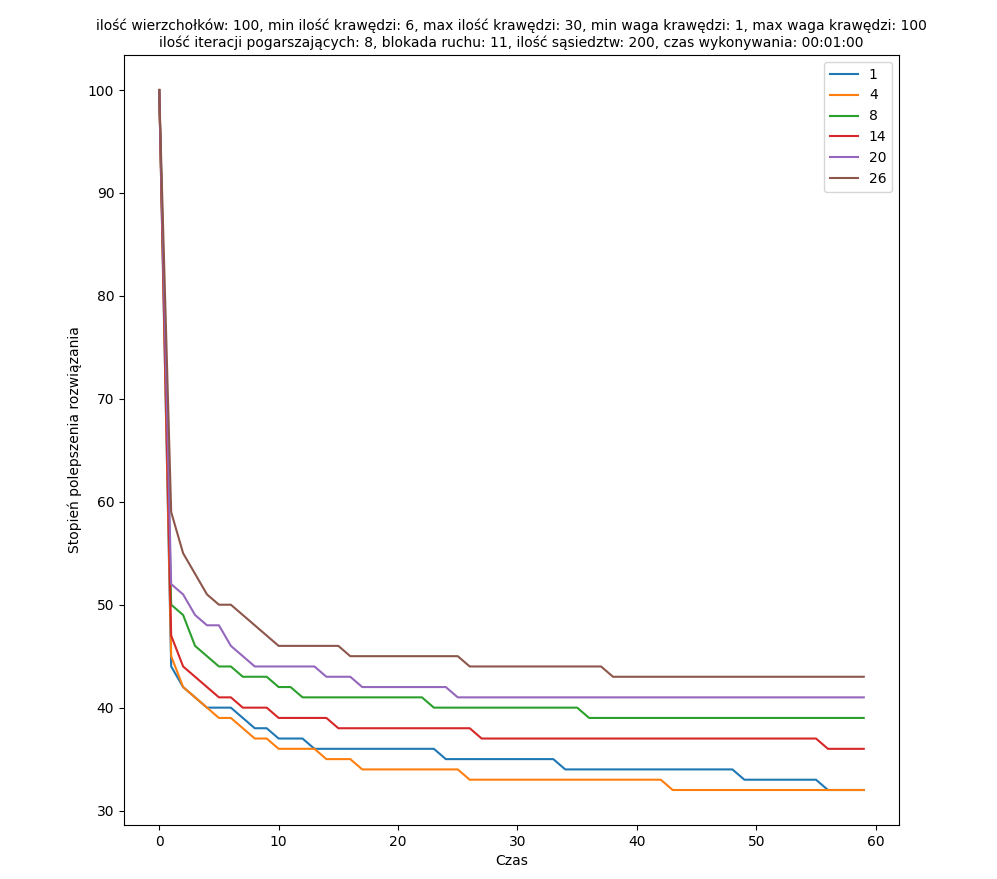
\includegraphics[scale=0.6]{pogorszenie_wykres.png}
  }
\end{center}


\section{Podsumowanie}
No jest wszystko w porządku, jest dobrze, dobrze robi, dobrze wszystko jest w porządku.
Jest git pozdrawiam całą bioinformatykę, dobrych chłopaków i niech sie to trzyma.
Dobry kod leci.


\end{document}